\begin{pa} \label{PA:10.2} Let's return to the function we considered
  in Preview Activity \ref{PA:9.1}.  Suppose we take out a \$18,000
  car loan at interest rate $r$ and we agree to pay off the loan in
  $t$ years.  The monthly payment, in dollars, is
  $$
  M(r,t) =
  \frac{1500r}{1-\left(1+\frac{r}{12}\right)^{-12t}}.
  $$

  \ba
  \item What is the monthly payment if the interest rate is $r=3\% =
    0.03$, and we pay the loan off in $t=4$ years?

  \item Suppose the interest rate is fixed at $r=3\%=0.03$.  Express $M$ as a function $f$ of $t$ alone using $r=0.03$. That is, let $f(t) = M(0.03, t)$. Sketch the graph of $f$ on the left of
    Figure \ref{F:10.2.preview.1}.  Explain the meaning of the function $f$.

    \begin{figure}[ht]
      \begin{center}
        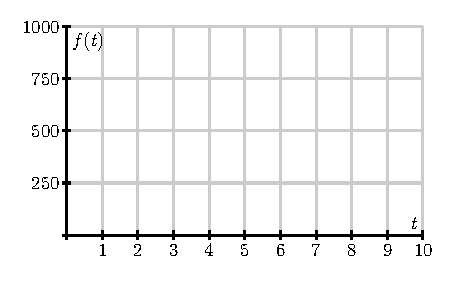
\includegraphics{figures/fig_10_2_preview_1.eps}
        \hspace*{20pt}
        \includegraphics{figures/fig_10_2_preview_2.eps}
        \caption{The graphs of $f(t)= M(0.03, t)$ and $g(r) = M(r,4)$.}
        \label{F:10.2.preview.1}
      \end{center}
    \end{figure}

  \item Find the instantaneous rate of change $f'(4)$ and state the units on
    this quantity.  What information does $f'(4)$ tell us about our
    car loan?  What information does $f'(4)$ tell us about the graph
    you sketched in (b)? 

  \item Express $M$ as a function of $r$ alone, using a fixed time of $t=4$.  That is, let $g(r) = M(r, 4)$. Sketch the graph of $g$ on the right of
    Figure \ref{F:10.2.preview.1}.  Explain the meaning of the function $g$.

  \item Find the instantaneous rate of change $g'(0.03)$ and state the units on
    this quantity.  What information does $g'(0.03)$ tell us about our
    car loan?  What information does $g'(0.03)$ tell us about the graph
    you sketched in (d)? 

    \ea


\end{pa} 

\begin{activitySolution}
 \ba
  \item If the interest rate is $r=3\% = 0.03$, and we pay the loan off in $t=4$ years, then the monthly payment is
  \[M(0.03,4) =   \frac{1500(0.03)}{1-\left(1+\frac{0.03}{12}\right)^{-12(4)}} \approx 398.42.\]

  \item If $r$ is fixed at $r=0.03$, then $M$ is a function of $t$ alone and 
\[f(t) = M(0.03,t) =  \frac{1500(0.03)}{1-\left(1+\frac{0.03}{12}\right)^{-12t}} = \frac{45}{1-1.0025^{-12t}}.\]
. The function $f$ tells us the monthly payment on a loan at different durations of time if the interest rate is fixed at $3\%$. 

  \item Using techniques from single variable calculus we have 
\[f'(t) = -\frac{(45)(12)1.0025^{-12t}\ln(1.00025)}{\left(1-1.0025^{-12t}\right)^2}.\]
So 
\[f'(4) \approx -84.54 \ \frac{\text{dollars}}{\text{year}},\]
which tells us that if we keep the interest rate constant at $3\%$, for every one year increase in the duration of the loan from 4 years there is an approximate decrease in the monthly payment of approximately 84.54 dollars. The quantity $f'(4)$ also tells us the slope of the line tangent to the graph of $f$ at $t=4$. 

  \item If $t$ is fixed at $t=4$, then $M$ is a function of $r$ alone and 
\[g(r) = M(r,4) = \frac{1500r}{1-\left(1+\frac{r}{12}\right)^{-12(4)}} = \frac{1500r}{1-\left(1+\frac{r}{12}\right)^{-48}}.\]
. The function $g$ tells us the monthly payment on a loan at different interest rates if the duration of the loan is fixed at 4 years.


  \item Using techniques from single variable calculus we have 
\[g'(r) = \frac{1500\left(1-\left(1+\frac{r}{12}\right)^{-48}\right) - 1500r\left(-48\left(1+\frac{r}{12}\right)^{-49}\right)\left(\frac{1}{12}\right)}{\left(1-\left(1+\frac{r}{12}\right)^{-48}\right)^2}.\]
So 
\[g'(0.03) \approx 795.54 \ \frac{\text{dollars}}{\text{\%}},\]
which tells us that if we keep the duration of the loan constant at 4 years, if we increase the interest rate by 1 from a rate of 3\%, the monthly payment on the loan increases by approximately \$795.54. The quantity $g'(0.03)$ also tells us the slope of the line tangent to the graph of $g$ at $r=0.03$. 

    \ea
  

\end{activitySolution}
\afterpa 